% 片面印刷用
%\documentclass[oneside,a4j]{ltjsarticle}
% 両面印刷用
\documentclass[twoside,a4j]{ltjsarticle}

\newcommand{\論文題目}{観光案内アプリにおける\\PWA活用に関する検討}
\newcommand{\英文題目}{A Study on the Use of PWA in \\Tourist Information Applications}
\newcommand{\学籍番号}{1038330}
\newcommand{\クラス名列番号}{4EP1-25}
% 名字と名前の間に半角スペースを入れる
\newcommand{\氏名}{笹川 尋翔}    

\newcommand{\年度}{5}
\newcommand{\提出日}{\和暦{}\today}
\newcommand{\指導教員}{坂本 真仁 講師}
\usepackage{sbase}

\begin{document}

\pagestyle{empty}
\vspace{10cm}
{\Large\bfseries
\noindent
令和\年度{}年度\ プロジェクトデザイン$\textrm{I\hspace{-.15em}I\hspace{-.15em}I}$ プロジェクトレポート\\
金沢工業大学\ 工学部\ 情報工学科\\

\vspace{4cm}
{\Huge\bfseries
\begin{center}
\論文題目
\end{center}
}
{\bfseries
\begin{center}
\英文題目
\end{center}
}

\vspace{6cm}
\begin{flushright}
\begin{tabular}{rl}
  学\hfill{}籍\hfill{}番\hfill{}号:
  & \学籍番号  \\
  ク\hfill{}ラ\hfill{}ス\hfill{}名\hfill{}列\hfill{}番\hfill{}号:
  & \クラス名列番号  \\
  氏\hfill{}名:
  & \氏名      \\
  提\hfill{}出\hfill{}日:
  & \提出日    \\
  指\hfill{}導\hfill{}教\hfill{}員:
  & \指導教員  \\
\end{tabular}
\end{flushright}
}

\clearpage
%%%%% 両面印刷の場合に表紙の裏を白紙にする
%%%%% 差し替えたときに目次を表紙の裏にしないため
%\thispagestyle{empty}
\hspace{5mm}
\clearpage
\noindent {\huge{概要}}\\ \vspace{5mm}

{\large{
% 500文字程度で概要を述べる
% 背景、目的、方法、結果、結果がどのような意味を持つのかを説明する文を含める
地域や所得によって十分な通信環境が確保できない人々が依然として存在し、高いユーザビリティーを実現することが困難である。安価な電子機器であるモバイル端末の需要が大きいため、特にモバイル端末のユーザビリティーを改善することが重要である。これを実現するための手段として、PWA(Progressive Web Apps)が注目されている。初めに、モバイルネイティブな観光案内アプリを比較対象として、PWAにおいてWeb標準のAPIを利用した場合のユーザビリティーの変化を考察した。次に、観光名所を地図にマッピングするWebアプリにPWAを組み込み、Lighthouseとネットワークスロットリングを使用してPWAのパフォーマンスを調査した。その結果、モバイルネイティブな観光案内アプリに実装されている機能の多くはPWAを利用したアプリにおいても実装可能であり、キャッシュ管理を行うことでパフォーマンスの低下を抑えられることが示された。これらの結果から、観光案内アプリにおいてPWAを利用した場合は、通信インフラや財政的な制約を受ける環境においても高いユーザビリティーを実現できると考えられる。
\vfill
\noindent {\huge{実施報告}}\\ \vspace{5mm}

{\bfseries{活動履歴}}
\begin{center}
\begin{tabular}{rlr} \hline
  \multicolumn{1}{c}{ {\bfseries {期間} }} &
  \multicolumn{1}{c}{ {\bfseries {活動内容} }} &
  \multicolumn{1}{c}{ {\bfseries {活動時間[h]} }}
    %% 期間 & 活動内容 & 活動時間[h]

\\ \hline
4月 & 研究で用いる端末の環境構築 & 41.0 \\
5月 & 研究計画の見直しと関連研究の調査 & 30.5 \\
6月 & 関連研究の調査と新しい研究計画に基づいた資料の作成 & 45.5 \\
7月 & 関連研究の調査と線形代数の勉強 & 35.5 \\
8月 & 研究の関連技術の勉強と中間発表用の資料の作成 & 37.5 \\
9月 & 研究の参考文献の調査 & 36.5 \\
10月 & システムの評価方法の策定 & 53.0 \\
11月 & 検証用のシステムの作成とパフォーマンスの測定 & 61.5 \\
12月 & システムの評価方法の見直し & 55.0 \\
1月  & 卒論と卒論の予稿の執筆 & 29.5 \\
\\ \hline


\end{tabular}
\end{center}
}}
\clearpage
\pagestyle{headings}
\pagenumbering{roman}
\setcounter{page}{1}
%%% 本文中では clearpageを使用してはならない
%%%%%%%%%%%%%%%%%%%%%%%%%%%%%%% ここまで表紙
\tableofcontents

% 以下の目次は不要であれば消す
% 図目次
\listoffigures
% 表目次
\listoftables
% ソースコード目次
\lstlistoflistings

\clearpage
\pagenumbering{arabic}
\setcounter{page}{1}

%% ここから本文を書く

\section{初めに}
\label{section:初めに}
通信インフラの整備状況は地域間で大きく異なる。例えば、モバイルネットワークの世代別のシェアを見ると、世界では2022年時点で4Gネットワークが88\%を占めるが、アフリカでの4Gネットワークの普及率は50\%、アラブ諸国では76\%となっている~\cite{ITU2022FactsAndFigures}。所得別で見ると低中所得以上の人々の間では比較的4Gネットワークの普及率が高いが、低所得の人々の間の普及率は34\%と低い値を示している。その他には、都市と地方の間にも同様の格差が残っていることが指摘されている。これらのデータは何を示唆しているのだろうか?
\subsection{背景}
\label{subsection:背景}
\subsubsection{モバイルネットワークの普及率の違い}
\label{subsubsection:モバイルネットワークの普及率の違い}
通信インフラへの投資が、モバイル通信システムの新しい世代の普及率に影響を及ぼしていることが指摘されている~\cite{Forge2020FormingA5GStrategyForDevelopingCountries}。通信インフラはモバイル通信サービスやオンラインサービスの基礎であるため、国々の間で激しい競争が行われているが、経済規模の違いから発展途上国や地方自治体は投資される側において不利である。膨大な予算を確保しやすい先進国や中央自治体の方がより魅力的な投資政策を立てられるためである。

他方で、通信システムを整備する組織の1つであるMNO(Mobile Network Operator)は、既にある通信設備の維持をしながら新しいモバイルネットワーク技術に多額の資金を投資する必要があるため、ある程度のリスクを抱えており、政府からの支援によって投資への積極性が左右されやすい。最近ではオンラインサービスを運営するMNOも登場しており、市場規模が拡大するにつれて明確な投資判断を下すために考慮するべき要素がますます増えている。

モバイル通信システムの世代が新しくなるにつれ、モバイル通信技術を導入するための費用が増加する傾向にある。例えば、モバイル通信システムの世代が新しいほど使用する周波数帯が高くなる傾向にあるが、これは1つの基地局が対応できる通信範囲が狭くなることを意味する。これにより、特定のカバレッジを確保する場合にかかる基地局などの設備費用が増加する。

さらに、高速な通信規格においては、5Gの要件であるeMBB(enhanced Mobile Broadband)、mMTC(massive Machine Type Communication)、uRLLC(Ultra-Reliable and Low Latency Communications)のような厳しい基準が定められており、開発に求められる技術が複雑化している。これは人件費の増加を招くため、モバイル通信技術を導入する際の1つの障壁となっている。

新しいモバイル通信技術はより高速なネットワークを提供するため、より多くの動画コンテンツに対応し、新しい市場や需要を産出する可能性があるが、その一方で現在の市場やエコシステムを大きく変える可能性もある。発展途上国や地方自治体は先進国や中央自治体に比べて受け取る投資額が少ないため、需要がどのくらいあるのかが明確ではない、新しいモバイル通信技術の開発や導入に消極的である。
\subsubsection{PWAの登場}
\label{subsubsection:PWAの登場}
通信技術の開発や通信インフラの整備状況は様々な要因の影響を受ける。これらの要因により十分な通信環境が確保できない地域に対してもユーザビリティーが高いサービスを提供することが必要である。特に、モバイル端末は安価である一方で、利用時には移動体通信が行われるため通信環境が変化しやすく、一定のユーザビリティーを確保することが難しい。このような問題を解決するために提案されている技術がPWA(Progressive Web Apps)である。

PWAはモバイルネイティブアプリに代表される、プラットフォーム固有のアプリのユーザビリティーを提供するWebの技術である。通常のWebアプリでは柔軟なキャッシュ管理ができないため、Webページの読み込み速度をキャッシュレベルで改善するための仕組みが複雑である。また、常にオンラインでアクセスする必要があるため、通信環境の地理的な制約を受けることがある。PWAを活用することでこれらの問題を解決できる。PWAを構成する要素をいくつか示す。

Web Application ManifestはWebアプリの情報を提供するJSONテキストファイルである。プラットフォーム固有のアプリが持っている、名前、説明、アイコン画像などのメタデータを記述する。必要な情報を記述することで、インストール時や起動時のUIを制御することもできる。開発者はWeb Application Manifestを使用することでユーザーにアプリの正確な情報を提示できるようになる。

Service WorkerはWeb Workerと呼ばれる仕組みの1つで、Webアプリ間、ブラウザー間、ネットワーク間でプロキシーサーバーとして動作する。オリジンサーバーへのネットワークリクエストを遮断し、ネットワークの利用状況に応じてオリジンサーバーの代わりにWebブラウザに対してネットワークレスポンスを返却することで、オフラインの際にもWebアプリを使用できるようにする。

PWAはWebアプリであるため、モバイル端末の一部のAPIにアクセスするためにはWeb APIを使用する必要がある。例えば、カメラ、マイク、位置情報、通知、端末の向きが挙げられる。Service Workerを制御する際にもWeb APIを使用する。一部のWeb APIは安全性が高いプロトコルであるHTTPSでのみ動作し、Web APIの対応状況はWebブラウザー間で異なることから、現在の対応状況や懸念点を考慮した上で、使用するものを決めることが重要である。PWAにおいて使用することが多いWeb APIや、Web APIの懸念点は後述する。

アプリは通常、コンテンツとそれを格納するUIからなる。App Shellはコンテンツを格納するUI(シェル)をコンテンツとは別にキャッシュすることで、アプリをオフライン環境で快適に動作させるためのアーキテクチャである。UIをコンテンツから分離することで読み込みが高速になり、3Gなどの低速な通信環境での読み込みの遅延を改善できる。

App Shellに基づいてキャッシュされる可能性があるネットワークリクエストはService Workerで制御される。また、Web APIを使用することで、シェルに加えてホーム画面への追加やプッシュ通知などの他の機能を追加できる。App Shellを採用することで、Webアプリで得られるユーザビリティーを、プラットフォーム固有のアプリで得られるユーザビリティーに近づけられる。
\subsubsection{位置情報市場の拡大とモバイルデータトラフィックの増加}
\label{subsubsection:位置情報市場の拡大とモバイルデータトラフィックの増加}
屋外の位置情報に関連する市場の規模は、国内では2025年度までに約1,900億円に拡大すると予想されている~\cite{MIC2023InformationStatistics}。位置情報は、地図、カーナビゲーション、マーケティング、タクシーの配車、ゲーム、家族や友人と位置情報を共有するアプリなどで活用されている。これらのサービスによって位置情報技術の認知度がより向上し、その認知度の高まりが位置情報市場の拡大を支えていると考えられる。

世界のモバイルデータトラフィックは2023年第2四半期から第3四半期にかけて前四半期比で7\%増加している~\cite{EricssonNovember2023MobilityReportDataAndForecasts}。モバイル通信システムの世代の移行が進んでいることや、画像、音声、動画などのコンテンツのアップリンクやダウンリンクのデータトラフィックが増加していることがこの要因である。動画コンテンツの視聴の増加が契約当たりの平均データ量の増加に関連していることから、配信されるコンテンツの種類の変化がモバイルデータトラフィックの増加に大きい影響を及ぼしていると考えられる。

このような背景を踏まえ、PWAの活用方法を検討する題材として観光案内を取り上げることにした。観光案内アプリは位置情報を使用する機会が多く、画像、音声、動画といったデータ量が大きいコンテンツを配信することが多いという特徴がある。

\subsection{目的}
\label{subsection:目的}
現在配信されている観光案内アプリに実装されている機能を調査し、観光案内アプリにPWAを導入する際の機能面の課題を明らかにする。関連研究で行われていたアプリのパフォーマンスの評価方法の問題点を指摘し、アプリのパフォーマンスをより正確に計測するための方法を示す。その方法を用いて、Service Workerのキャッシュ戦略を活用した場合の観光案内アプリのパフォーマンスを計測し、その戦略がどの程度効果的であるのかを示す。新たに提案したパフォーマンスの計測方法を用いてパフォーマンスを評価した場合に生じる問題点を指摘し、どのような改善が求められるのかを示す。
\subsection{構成}
\label{subsection:構成}
~\autoref{section:関連研究}では、PWAの性質、パフォーマンス、役割を論じている研究を紹介し、関連研究でまだ明らかにされていないことや、関連研究の課題を説明する~\autoref{section:研究内容}では、PWAを用いた観光案内アプリのパフォーマンスを評価する方法を述べる。~\autoref{section:評価}では、PWAを用いた観光案内アプリでの、Web APIの有用性とService Workerのパフォーマンスを評価する。~\autoref{section:まとめ}では、観光案内アプリにおけるPWAの有用性を評価し、観光案内アプリにPWAを導入する上での課題を考察する。その後にこの研究の目的を振り返り、研究で明らかになったことや今後さらなる研究が必要なことをまとめる。Service Workerのパフォーマンスを計測する際に使用したプログラムとそのプログラムの実行環境を付録に示す。

\section{関連研究}\label{section:関連研究}
%\begin{itemize}
%  \item PWAの構成要素
%  \begin{itemize}
%    \item PWAを構成する要素を考察した研究を提示する
%  \end{itemize}
%  \item クロスプラットフォーム開発におけるPWA
%  \begin{itemize}
%    \item クロスプラットフォーム開発におけるPWAを考察した研究を提示する
%    \item 関連研究と自分の研究を比べた場合の相違点を述べる
%  \end{itemize}
%\end{itemize}
関連研究としては、PWAを構成する要素の性質を調査したもの、PWAとモバイルアプリとの比較によって有用性を評価したもの、PWAの開発方法に着目し、クロスプラットフォーム開発との特徴の違いを整理したものなどがある。それぞれの概要を説明し、関連研究における課題を整理する。
\subsection{PWAの構成要素とその性質}\label{subsection:PWAの構成要素とその性質}
PWAの構成要素にはApp Shell、Service Worker、Web Application Manifestがあり、それぞれの性質は以下の通りである~\cite{Tandel2018ProgressiveWebApps}。
\subsubsection{App Shellの性質}\label{subsubsection:App Shellの性質}
\begin{itemize}
    \item パフォーマンスが高い
    \begin{itemize}
      \item キャッシュされたコンテンツを利用することで高速にページを読み込めるため、通常のWebアプリと比べてパフォーマンスが高い。これはアプリに再びアクセスした際にページが即座に読み込まれることを意味する。
    \end{itemize}
    \item ネイティブアプリに近い操作性を実現
    \begin{itemize}
        \item Cache APIを利用することでオフライン環境でも動作する。PWAが考案される前は、ネイティブアプリのみがオフラインアクセスをサポートしていた。PWAによってネイティブアプリに近い操作性を実現するWebアプリが登場したことで、Webアプリの多様化が進んだ。
    \end{itemize}
    \item データの使用効率が高い
    \begin{itemize}
        \item UIをキャッシュするためページ遷移を行う際のデータ使用量が削減される。これによってデータの使用効率が高くなり、より少ないデータ使用量でページをレンダリングできるようになる。
    \end{itemize}
\end{itemize}
\subsubsection{Service Workerの性質}\label{subsubsection:Service Workerの性質}
\begin{itemize}
    \item オフラインアクセスを提供
    \begin{itemize}
        \item キャッシュしたネットワークレスポンスを使用してオフラインアクセスを提供できる。通信が不安定な環境でもアプリを利用できるようになるため、ユーザー体験が向上し、ユーザーに新たな価値を提供できるようになる、
    \end{itemize}
    \item プッシュ通知を提供
    \begin{itemize}
        \item ユーザーのモバイル端末やデスクトップ端末に直接送信されるメッセージであるプッシュ通知を提供できる。プッシュ通知を効果的に活用することで、アプリの利用を促進してコンバージョン率を向上させたり、行動パターンをより詳細に分析したりできるようになる。
    \end{itemize}
    \item バックグラウンドでコンテンツを更新
    \begin{itemize}
        \item Periodic Background Synchronization APIを用いることでバックグラウンドでコンテンツを更新できる。コンテンツを同期する際にユーザーの直接的な操作が不要になり、ユーザーに常に最新の情報を提供できる。
    \end{itemize}
    \item 柔軟なキャッシュ制御
    \begin{itemize}
        \item 一部のコンテンツのみをキャッシュしたり、一定の時間間隔でキャッシュを更新したりできるため、Cache Storageの使用量を削減してアプリのサイズを小さくしたり、古いコンテンツがキャッシュされたままになるのを回避できる。
    \end{itemize}
\end{itemize}
\subsubsection{Web Application Manifestの性質}\label{subsubsection:Web Application Manifestの性質}
\begin{itemize}
    \item アプリに関する情報を提供
    \begin{itemize}
        \item アプリの名前、説明、作者、アイコンのパスなどの情報を提供できる。これらのメタデータをWebアプリに追加することで、Webアプリを特定のプラットフォームに適合させられる。
    \end{itemize}
\end{itemize}
\subsubsection{PWAの構成要素とその性質に関する研究の課題}
実際のアプリでは、PWAが理想とする振る舞いを必ずしも実現できるとは限らない。例えば、バックグラウンドでのコンテンツの更新をサポートしている主なWebブラウザーは2023年11月時点でGoogle ChromeとMicrosoft Edgeのみであり、バックグラウンド同期に関する懸念も表明されている(詳しくは後述する)。また、Webブラウザー間でPWAの実装が異なるため、それを考慮する必要もある。


\section{研究内容}\label{section:研究内容}
観光案内アプリにPWAを導入することを想定して調査や分析を行う。まずはPWAと深い関わりがあるWeb APIの、PWAにおける有用性を調査する。続いてService Workerのパフォーマンスを評価する。
\subsection{PWAにおけるWeb APIの有用性の調査}\label{subsection:PWAにおけるWeb APIの有用性の調査}
Web APIはPWAをプラットフォーム固有のアプリ(ネイティブアプリ)に近づけるために不可欠な技術である。ネイティブアプリの機能の多くはSDK(Software Development Kit)により提供されている。SDKは、特定のフレームワークやプラットフォーム上にアプリケーションを構築するために使用する開発ツールのセットである。Webアプリ開発では、SDKの代わりにWeb APIを使用できる。API(Application Programming Interface)はプログラム同士が相互に通信するための方法である。SDKと同様に、開発者が複雑な機能をより簡単に作成できるようにするために提供されており、APIを使用することで複雑なコードが抽象化され、構文がより簡潔になる。Web APIはこのAPIの1つであり、HTTPなどのWebの技術を利用したものである。Web APIにはいくつかの種類があるが、この論文では特に、WebブラウザーのAPIのうち、W3Cなどにより標準化されたものを扱うことにする。以後この論文では、Webブラウザーの標準化されたAPIという意味でWeb APIという語句を使用する。
\subsubsection{Web APIのWebブラウザー側の対応状況の調査}\label{subsubsection:Web APIのWebブラウザー側の対応状況の調査}
開発者が実際に特定のWeb APIを利用するためには、WebブラウザーがそのWeb APIに対応している必要がある。特に、シェアが大きいWebブラウザーの対応状況や、レンダリングエンジンが異なるWebブラウザー間の対応状況を把握することは、Webアプリのコンバージョンを高めたり、自由なWebを維持したりする上で重要である。主要なWebブラウザーのシェアや特徴は以下の通りである。なお、シェアはすべてのプラットフォームの2023年9月時点のデータを基に算出している~\cite{StatCounterBrowserMarketShare}。
\begin{itemize}
    \item Google Chrome
    \begin{itemize}
        \item シェア: 約63\%
        \item レンダリングエンジン
        \begin{itemize}
            \item HTML: Blink
            \item JavaScript: V8
        \end{itemize}
        \item チャンネル~\cite{GoogleChromeChannels}
        \begin{itemize}
            \item Stable
            \item Extended Stable
            \item Beta
            \item Dev
            \item Canary
        \end{itemize}
    \end{itemize}
    \item Safari
    \begin{itemize}
        \item シェア: 約20\%
        \item レンダリングエンジン
        \begin{itemize}
            \item HTML: WebKit
            \item JavaScript: Nitro
        \end{itemize}
        \item チャンネル~\cite{SafariChannels}
        \begin{itemize}
            \item Safari
            \item Beta
            \item Technology Preview
        \end{itemize}
    \end{itemize}
    \item Microsoft Edge
    \begin{itemize}
        \item シェア: 約5\%
        \item レンダリングエンジン
        \begin{itemize}
            \item HTML: Blink
            \item JavaScript: V8
        \end{itemize}
        \item チャンネル~\cite{MicrosoftEdgeChannels}
        \begin{itemize}
            \item Stable
            \item Extended Stable
            \item Beta
            \item Dev
            \item Canary
        \end{itemize}
    \end{itemize}
    \item Mozilla Firefox
    \begin{itemize}
        \item シェア: 約3\%
        \item レンダリングエンジン
        \begin{itemize}
            \item HTML: Gecko
            \item JavaScript: SpiderMonkey
        \end{itemize}
        \item チャンネル~\cite{MozillaFirefoxChannels}
        \begin{itemize}
            \item Firefox
            \item Extended Support Release(ESR)
            \item Beta
            \item Developer Edition
            \item Nightly
        \end{itemize}
    \end{itemize}
\end{itemize}
次に、前述した情報を踏まえ、Webブラウザー間におけるWeb APIの対応状況の違いを考える上で、着目するべき点を挙げる。まずは、Google Chromeのシェアとその他のWebブラウザーのシェアの間に大きな差があることを確認できる。次に、Google ChromeとMicrosoft Edgeの特徴が似ていることを確認できる。Microsoft EdgeはGoogle Chromeと同様にChromiumというWebブラウザーから派生しているためである。Web APIの対応状況についてもほとんど同じである。そこで、Google ChromeとMicrosoft Edgeは同一のWebブラウザーであるとみなし、よりシェアが大きいGoogle Chromeを調査対象とする。

続いて、HTMLのレンダリングエンジンの違いに注目する。まず、SafariはBlinkのフォーク元であるWebKitを利用している。そのため、SafariにはGoogle ChromeやMicrosoft Edgeと共通のコードベースが含まれる可能性がある。さらに、WebKitは独自のエコシステムを持っている。例えば、iOS上のWebブラウザーはWebKit以外のHTMLレンダリングエンジンを使用できない。これにより、iOS上のWebブラウザー間の機能の違いが少なくなり、iOSにデフォルトでインストールされているSafariの市場優位性が高まる。Mozilla Firefoxについては、シェアは少ないものの、WebKitから完全に独立したHTMLレンダリングエンジンであるGeckoを採用している。また、プライバシーを重視する傾向にあり、PWAに関連するWeb APIの策定に積極的であるGoogle Chromeとは対照的である。そのため、Google Chromeに加えてMozilla Firefoxも調査対象とする。

次に、Web APIのWebブラウザー側の対応状況を調べる際に参照する文献の候補を示す。Can I use…~\cite{CanIUse}は様々なWebブラウザーがサポートする機能を検索できるWebサイトである。CC BY 4.0ライセンスを採用し、コミュニティーがWebサイトの情報を更新している。これに加えて、より信ぴょう性が高い情報を得るために、それぞれのWebブラウザーベンダーが提供しているRelease notesを参照する。これは、新しいバージョンのソフトウェアをリリースする際に公表される、以前のバージョンからの変更点を示す文書である。また、より詳細な情報を入手するために、必要に応じてWebブラウザーベンダーのブログ記事を参照する。
\subsubsection{Web APIに対する意見や主張の調査}\label{subsubsection:Web APIに対する意見や主張の調査}
それぞれのWeb APIに対する意見や主張は、Web APIの有用性を測るための1つの指標となり得る。Web APIに対する意見や主張を表明するための文書としてはStandards Positionsがある。これは、Web標準の技術に対する開発コミュニティーの立場をまとめたものである。主な立場としては賛成(support、positive)、中立(neutral)、反対(oppose、negative)がある。GitHubなどのプラットフォーム上で、特定のWeb標準の技術に対する賛否の議論が行われ、その後に開発コミュニティーの代表者が立場を表明する。まずは、Standards Positionsでの立場やその根拠となる議論を調査し、Web APIの現在の有用性を評価する。さらに、Web APIに対する議論の方向性を基にWeb APIの将来の見通しを考察する。
\subsection{Service Workerのパフォーマンスの評価}\label{subsection:Service Workerのパフォーマンスの評価}
観光案内アプリでのService Workerのパフォーマンスを評価するためには、観光案内アプリに求められる機能を調査し、検証用のアプリを作成し、Service Workerのキャッシュパターンを考え、パフォーマンスを計測することが必要である。
\subsubsection{観光案内アプリに求められる機能の調査}\label{subsubsection:観光案内アプリに求められる機能の調査}
人々が観光案内アプリと聞いて思い浮かべるものは様々である。そこで、観光案内アプリに求められる機能を調査する。初めにGoogle検索エンジンを使用して都道府県名、「観光」、「アプリ」というキーワードで検索する。次に、最上位の検索結果から順に閲覧していき、観光案内アプリを見つける。そのアプリが配信中であれば、PCやスマートフォンで実際にそのアプリを使用してアプリに実装されている機能を調査する。
\subsubsection{検証用のアプリの作成}\label{subsubsection:検証用のアプリの作成}
一般的にWebアプリはフレームワークを使用して作成される。そのため、検証用のアプリを作成する際も同種のソフトウェアを使用する。HTMLの生成方法は大きく分けて2種類あり、どちらを採用するかを決める必要がある。まずは、それらの方法を説明する。

最も基本的なHTMLの生成方法としては動的な生成がある。ユーザーがページにアクセスするたびにサーバー側でHTMLファイルが生成される。動的な生成を使用すると、ユーザーから任意のパラメーターを受け取り、それに基づいてHTMLを生成できる。後述する静的な生成では、Webアプリのプログラムを変更するたびにHTMLを生成し直さなければならないが、動的な生成ではその必要がないため、最新の情報を素早くユーザーに届けられる。動的な生成はSSR(Server Side Rendering)という仕組みによって実現しており、通常、HTMLを動的に生成する場合は、WebサーバーとWebアプリサーバーが必要である。

もう1つの生成方法は静的な生成である。Webアプリを変更してデプロイする際にはビルドという処理が行われるが、静的な生成では、この処理を行う際にそれぞれのページのHTMLファイルが生成される。したがって、ユーザーが特定のページにアクセスした際にクライアントに返却されるHTMLの内容は、ビルドが更新されない限り常に同じである。静的な生成はSSG(Static Site Generator)という仕組みによって実現しており、HTMLを静的に生成する場合はWebサーバーが必要である。

前述したように、静的な生成ではWebアプリのプログラムを変更するたびにHTMLを生成し直さなければならないという短所があり、コンテンツ指向型のWebアプリで静的なHTML生成が用いられることは少ない。そこで、検証用のアプリの作成時はHTMLを動的に生成する方法であるSSRを使用する。

\subsubsection{Service Workerのキャッシュ戦略}\label{Service Workerのキャッシュパターン}
Service Workerのキャッシュパターンはキャッシュ戦略と呼ばれ、Service Workerを効果的に使用するために必要である。どのコンテンツをキャッシュするべきかはアプリの内容によって異なるため、キャッシュ戦略は無数にあるが、参考までにいくつか例を示す。

まずは、Service Workerのインストール時に全てのアセットをキャッシュする戦略がある。この戦略ではService Workerはアセットのキャッシュのみを返すため、HTMLなどのネットワークリクエストはService Workerを経由せず、キャッシュされない。

あるいは、全てのネットワークリクエストをService Workerに経由させる戦略もある。この戦略ではコンテンツは一切キャッシュされないが、常に最新のネットワークレスポンスを受け取れる。しかし、ユーザーがオフラインのときはWebアプリが機能しない。

このように、Service Workerはネットワークリクエストを仲介する役割を持つ。そのため、Service Workerを用いて一部のコンテンツのみをキャッシュすることもできる。キャッシュ対象のコンテンツの種類や範囲を変化させることでSerivce Workerのパフォーマンス評価を行うことにし、3種類のキャッシュ戦略を策定した。

1つ目はすべてのネットワークレスポンスをキャッシュする戦略である。この戦略では、HTML、CSS、JavaScript、画像、JSONなどのあらゆるネットワークレスポンスがService Workerによって全てキャッシュされる。同じページがもう1度読み込まれると、全てのネットワークレスポンスがキャッシュを利用するため、実質的にネットワークリクエストが発生しない。

2つ目はSame-Originのネットワークレスポンスをキャッシュする戦略である。この戦略ではWebアプリがデプロイされているドメイン(Same-Origin)に対するネットワークリクエストのみがキャッシュされる。同じページがもう1度読み込まれると、Same-OriginのネットワークレスポンスはCache Storageにあるキャッシュを利用し、Cross-Originのネットワークレスポンスはそのキャッシュを利用しない。

3つ目は画像をキャッシュする戦略である。観光案内アプリでは多くの画像が配信されるため、画像を積極的にキャッシュした際のパフォーマンスを知ることは、観光案内アプリでのPWAの有用性を評価する上で重要である。
\subsubsection{Service Workerのパフォーマンスの計測}\label{subsubsection:Service Workerのパフォーマンスの計測}
現在広く普及しているWebアプリの品質測定ツールとしてLighthouseがある。Lighthouseを使用すると、任意のページに対してパフォーマンス、ユーザー補助、PWA、SEOなどの監査を実施できる。今回はパフォーマンスに着目しているため、パフォーマンスの監査のみを実施する。より正確な指標を得るために、LighthouseのNodeモジュールを使用してモバイル端末での読み込みをエミュレートする。

Lighthouseのパフォーマンスの指標は0から100で表され、監査項目の条件を満たしているほど、すなわちページの品質が高いほど値が大きくなる。パフォーマンスの評価に役立つその他の指標としては以下のようなメトリクスがある。

\begin{itemize}
    \item First Contentful Paint(FCP)
    \begin{itemize}
        \item ページのナビゲーションが開始されてから、Webブラウザーがコンテンツの最初の部分をレンダリングするまでにかかる時間である。このコンテンツとはテキスト、画像、<svg>要素、白以外の<canvas>要素を指す。
    \end{itemize}
    \item Largest Contentful Paint(LCP)
    \begin{itemize}
        \item ページのナビゲーションが開始されてから、最も大きな画像またはテキストブロックをレンダリングするまでにかかる時間である。
    \end{itemize}
    \item Speed Index(SI)
    \begin{itemize}
        \item ページの読み込み中にコンテンツが視覚的に表示される速度である。ページを読み込む際に発生するフレーム間の視覚的な変化を計算し、SpeedlineというNodeモジュールを使用して点数を生成する。
    \end{itemize}
    \item Total Blocking Time(TBT)
    \begin{itemize}
        \item マクスのクリック、画面のタップ、キーボードの押下などのユーザー入力に対するページの応答がブロックされている合計時間である。
    \end{itemize}
    \item Cumulative Layput Shift(CLS)
    \begin{itemize}
        \item ページの読み込みの開始から終了までの間に発生したセッションウィンドウのうち、そのウィンドウ内のレイアウトシフトの累積値が最も大きいセッションウィンドウの測定値である。
    \end{itemize}
\end{itemize}

モバイル端末をエミュレートする際は、端末の幅、高さ、性能に加えてモバイル端末の通信環境もエミュレートする必要がある。しかし、4G以前のモバイル通信システムはIEEE 802.11acなどの広く普及している無線LANの標準規格に比べて通信速度が低いため、無線LANに接続した端末で、ネットワークエミュレーションを行わずにパフォーマンスを計測すると、実際のモバイル端末でのパフォーマンスを正確に計測できない可能性が高い。このような問題を回避するためにネットワークスロットリングを使用する。ネットワークスロットリングとはインターネットの速度を意図的に低下させ、低帯域の状態をエミュレートすることである。ネットワークスロットリングには以下の4種類がある。

\begin{itemize}
    \item シミュレートされたスロットリング
    \begin{itemize}
        \item スロットリングされていない最初の読み込みで観察されたデータに基づいてページの読み込みをシミュレートする。高速であるが一部のサイトではスロットリングの正確性が低い。
    \end{itemize}
    \item リクエストレベルのスロットリング
    \begin{itemize}
        \item ネットワークリクエストごとにスロットリングを行う。スロットリングの正確性はSimulated throttlingと同じ程度である。
    \end{itemize}
    \item プロキシーレベルのスロットリング
    \begin{itemize}
        \item HTTPサーバーを経由したTCPやUDPのネットワークリクエストごとにスロットリングを行う。
    \end{itemize}
    \item パケットレベルのスロットリング
    \begin{itemize}
        \item パケットごとにスロットリングを行う。このスロットリングを使用することで最も正確なネットワークシミュレーションを行える。
    \end{itemize}
\end{itemize}

この研究では、より正確なデータを得るために、パケットレベルのスロットリングを使用してパフォーマンスを計測する。

\section{評価}
\label{section:評価}
\subsection{Service Workerのパフォーマンス}
\label{subsubsection:Service Workerのパフォーマンス}
Lighthouseとネットワークスロットリングを使用して、それぞれの都道府県の観光地図を読み込んだ際のパフォーマンスを計測した。キャッシュ戦略ごとのパフォーマンス指標の値の平均を図~\ref{figure:Service Workerを使用しなかった場合のパフォーマンス}、~\ref{figure:画像をキャッシュした場合のパフォーマンス}、~\ref{figure:Same-Originのネットワークレスポンスをキャッシュした場合のパフォーマンス}、表~\ref{table:全てのネットワークレスポンスをキャッシュした場合のパフォーマンス}に示す。
\begin{figure}
  \centering
  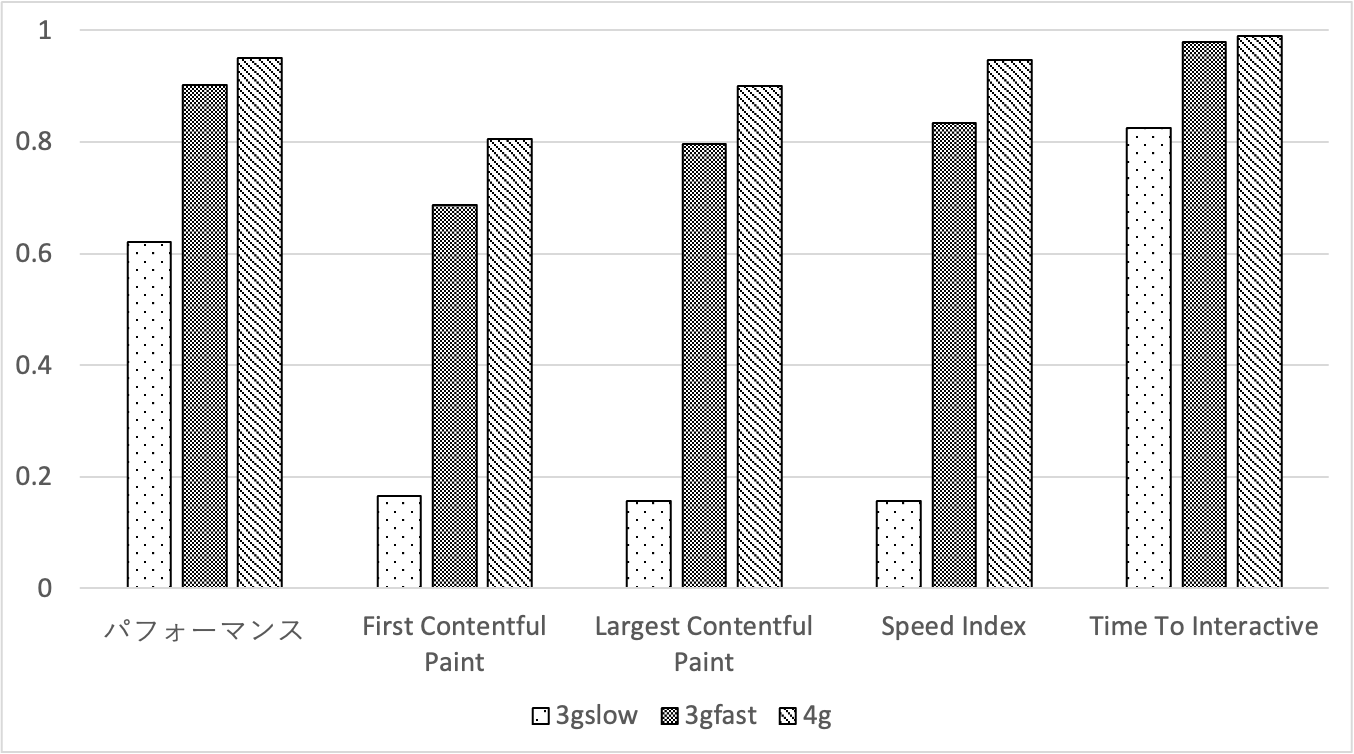
\includegraphics[width=0.9\textwidth]{images/without_service_worker.png}
  \caption{Service Workerを使用しなかった場合のパフォーマンス}\label{figure:Service Workerを使用しなかった場合のパフォーマンス}
\end{figure}
\begin{table}
  \caption{全てのネットワークレスポンスをキャッシュした場合のパフォーマンス}
  \label{table:全てのネットワークレスポンスをキャッシュした場合のパフォーマンス}
  \centering
  \begin{tabular}{|p{15em}|p{5em}|p{5em}|p{5em}|}
    \hline
    & 3gslow & 3gfast & 4g \\ \hline
    パフォーマンス & 1 & 1 & 1 \\ \hline
    First Contentful Paint & 1 & 1 & 1 \\ \hline
    Largest Contentful Paint & 1 & 1 & 1 \\ \hline
    Speed Index & 1 & 1 & 1 \\ \hline
    Total Blocking Time & 1 & 1 & 1 \\ \hline
    Cumulative Layout Shift & 1 & 1 & 1 \\ \hline
  \end{tabular}
\end{table}
\begin{figure}
  \centering
  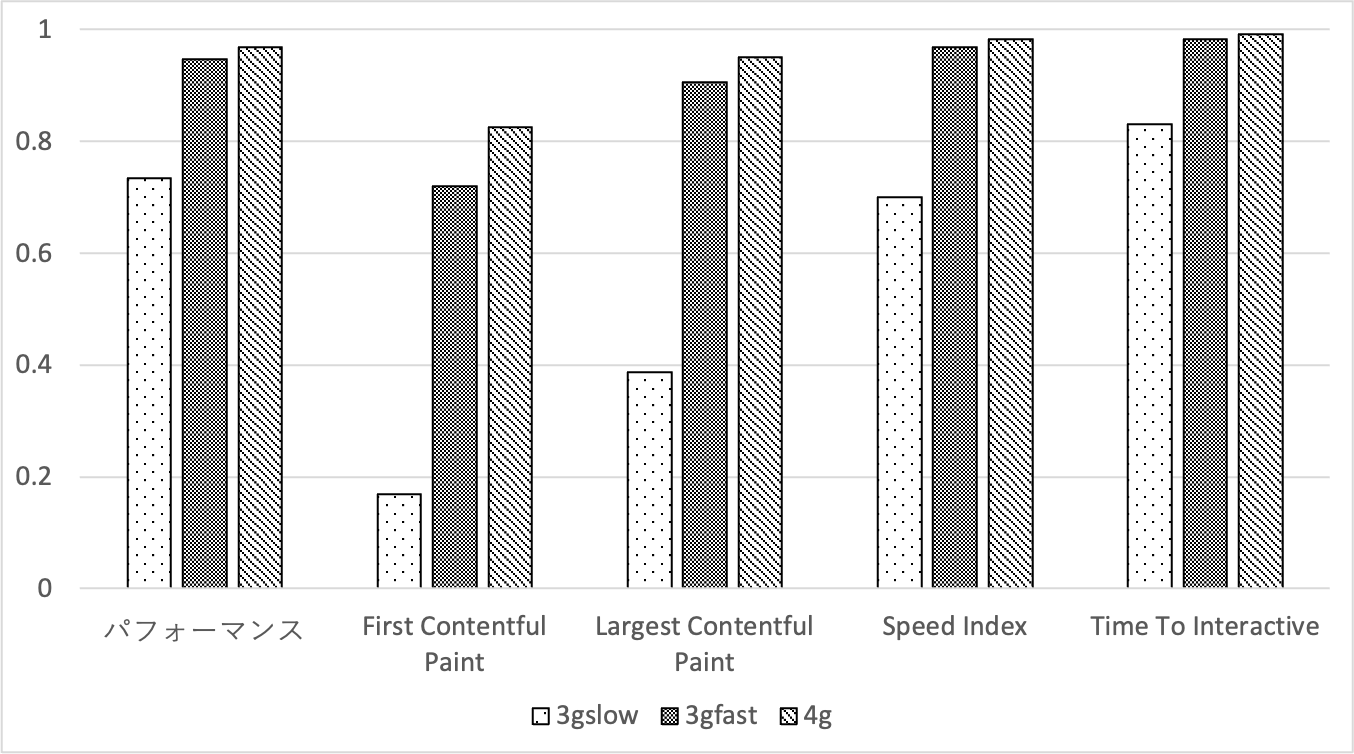
\includegraphics[width=0.9\textwidth]{images/service_worker_cache_images.png}
  \caption{画像をキャッシュした場合のパフォーマンス}\label{figure:画像をキャッシュした場合のパフォーマンス}
\end{figure}
\begin{figure}
  \centering
  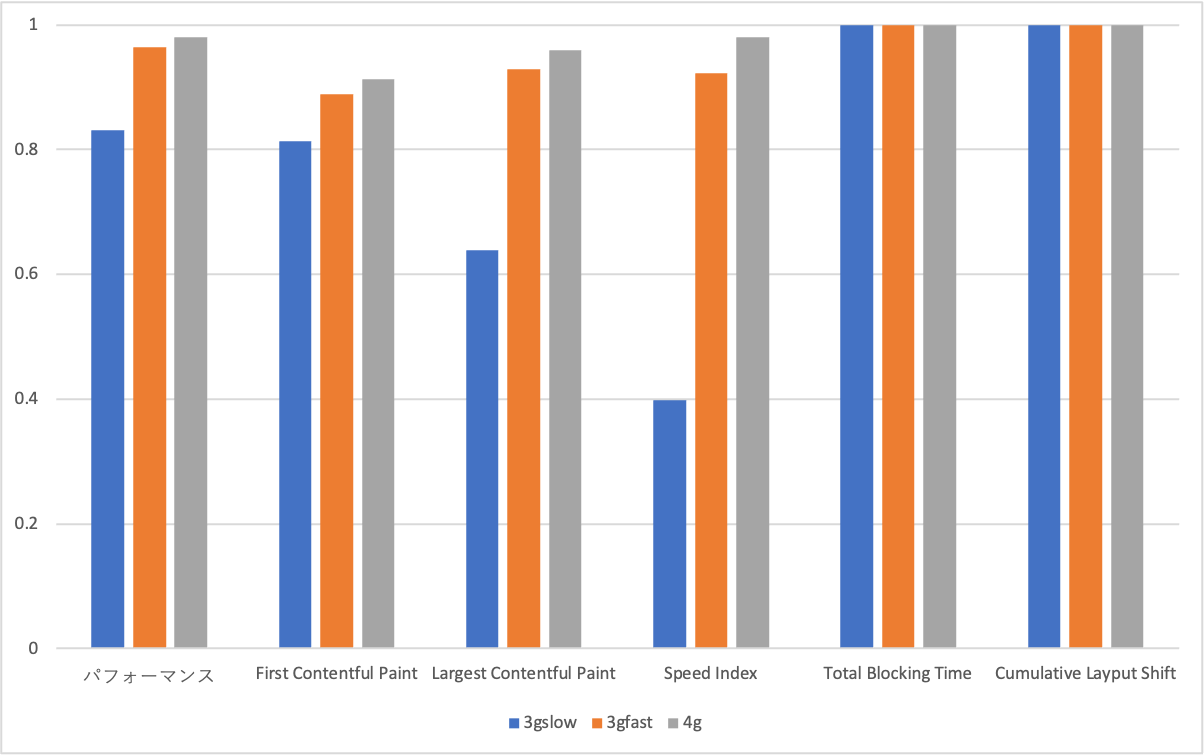
\includegraphics[width=0.9\textwidth]{images/service_worker_cache_same_origin.png}
  \caption{Same-Originのネットワークレスポンスをキャッシュした場合のパフォーマンス}\label{figure:Same-Originのネットワークレスポンスをキャッシュした場合のパフォーマンス}
\end{figure}
いずれの場合もTBTとCLSは1である。4g、3gfast、3gslowの順でパフォーマンス指標の値が大きい傾向にある。全てのネットワークレスポンスをキャッシュした場合は3gslow、3gfast、4gのいずれの場合も全ての指標の値は1である。画像をキャッシュした場合はFCPが最も通信速度の低下の影響を受けやすく、SIが最もその影響を受けにくいことが分かる。逆に、Same-Originのネットワークレスポンスのキャッシュした場合はSIが最も通信速度の低下の影響を受けやすく、SCPが最もその影響を受けにくいことが示されている。

3gfastに比べてアップリンクがおよそ12倍、ダウンリンクがおよそ6倍である4gプロファイルを使用した場合であってもほとんどのパフォーマンス指標の値は1未満である。全体的に見ると、3gslowと3gfast間のパフォーマンス指標の値の増加率は3gfastと4g間の増加率よりも大きい。

\section{まとめ}\label{section:まとめ}
%\begin{itemize}
%  \item Web API
%  \begin{itemize}
%    \item モバイル端末へのアクセス
%    \begin{itemize}
%      \item モバイル端末の主要な機能にアクセスするためのWeb APIの対応状況や懸念点を述べる
%    \end{itemize}
%    \item バックグラウンドでの動作
%    \begin{itemize}
%      \item バックグラウンドでWebアプリを動作させるために必要なWeb APIの短所と課題を述べる
%    \end{itemize}
%  \end{itemize}
%  \item Service Worker
%  \begin{itemize}
%    \item キャッシュ制御
%    \begin{itemize}
%      \item Service Workerを利用することでキャッシュを柔軟に制御でき、古い世代のモバイル通信システムを使用した場合や一部のコンテンツのみをキャッシュした場合でもパフォーマンスの低下を抑えられることを述べる
%    \end{itemize}
%  \end{itemize}
%\end{itemize}
\subsection{観光案内アプリにおけるPWAの評価と課題}\label{subsection:観光案内アプリにおけるPWAの評価と課題}
観光案内アプリはコンテンツの配信を中心とするサービスである。現在配信されている観光案内アプリに実装されている機能の多くは先にユーザーからのアクションを必要とするため、Background Fetch APIやBackground Synchronization APIを使用したバックグラウンドでのコンテンツの取得や更新の需要はまだ小さいことが分かる。これらのWeb APIを使用したバックグラウンド処理はWebページの再読み込みの手間やコンテンツのダウンロードの手間を削減するが、ユーザーがその処理の流れを理解しにくいためプライバシー上の懸念がある。

一方で、現在配信されている観光案内アプリにおいては、GPSなどを使用した位置情報の取得が普及していることから、位置情報は観光地図などの機能を適切に動作させるために不可欠な仕組みであると言える。この仕組みをPWAに取り入れるためにはGeolocation APIを使用することが一般的である。アプリがGeolocation APIを使用してユーザーの位置情報にアクセスするためには、ユーザーがアプリに対してプロンプト経由で明示的にアクセスを許可する必要があり、かつユーザーにとってその流れが直感的であるため、観光案内アプリにおいて活用が期待される。

アプリの進化の歴史を踏まえると、アプリのインタラクティブ性は今後ますます高まると考えられる。前述したように、現在配信されている観光案内アプリの多くは受動的であり、アプリからユーザーへの積極的な情報発信が少ない。しかし、今後アプリのインタラクティブ化が進めば、ユーザーに適した観光名所の提案や、新しい観光名所の紹介がアプリのアクションをきっかけに行われるようになる可能性もある。このような機能がより一般的になれば、Push APIとNotifications APIを用いたプッシュ通知の価値が高まり、最終的にはPWAの有用性が向上するかもしれない。



\section*{謝辞}\addcontentsline{toc}{section}{謝辞}

%% まずは指導教員
この研究を行うにあたり,〇〇大学〇〇学部〇〇学科教授であり,指導教員の〇〇博士には多大なるご助言を賜りました.
方向性を見失いそうになった際も,適切に導いてくださいました.
研究を行う際も有益な情報などを頂き,研究の幅も広がりました.
感謝申し上げます.


%% 次に副査の先生や共同研究先の方々
〇〇大学〇〇学部〇〇学科准教授の〇〇博士には,学部生の頃からお世話になり,非常に多くのことを学ばせていただきました.深く感謝します.
さらに,〇〇大学〇〇学部〇〇学科の助教である〇〇博士には,かけがえのない多くのことをご教授して頂きました.研究に対する技術的な内容だけでなく,個人的な日々の相談にも幾度となく乗ってくださいました.感謝の意を表します.


%% 他の先生や研究室の仲間
〇〇大学〇〇学部〇〇工学科,〇〇研究室の〇〇先輩には,学
部生として研究を始めた頃からお世話になりました.長い期間悩んでいた問題が,〇〇先輩から頂いたアドバイスによって即時に解決した出来事は忘れることが出来ません.
加えて,研究の日々を共に過ごした同期であり,つらい時期も励まし合い,互いに切磋琢磨した〇〇研究室の〇〇氏,〇〇研究室の〇〇氏に感謝します.


%% 友人や家族
最後にこれまで長い間ずっと支えとなってくれた家族に深謝します.





\newpage

\bibliographystyle{junsrt}
\bibliography{reference.bib}

\section*{付録}\addcontentsline{toc}{section}{付録}
~\autoref{subsection:Service Workerのパフォーマンス}で使用したプログラムをソースコード~\ref{lst:Lighthouseを用いたパフォーマンスの計測}に示す。~\autoref{subsection:ユーザーの操作に基づいて読み込まれた画像の処理時間}で使用したプログラムをソースコード~\ref{lst:PuppeteerとResource Timing APIを用いたページ読み込み時の画像の読み込み時間の計測}、~\ref{lst:PuppeteerとResource Timing APIを用いたスクロール時の画像の読み込み時間の計測}、~\ref{lst:PuppeteerとResource Timing APIを用いたズーム時の画像の読み込み時間の計測}に示す。

\begin{lstlisting}[caption={Lighthouseを用いたパフォーマンスの計測},label={lst:Lighthouseを用いたパフォーマンスの計測}]
import fs from "fs";
import lighthouse, { Flags } from "lighthouse";
import * as chromeLauncher from "chrome-launcher";

const chrome = await chromeLauncher.launch({ chromeFlags: ["--headless"] });

const options: Flags = {
  logLevel: "info",
  output: "csv",
  port: chrome.port,
  onlyCategories: ["performance"],
  formFactor: "mobile",
  screenEmulation: {
    mobile: true,
    disabled: false
  },
  throttlingMethod: "devtools",
  throttling: {
    requestLatencyMs: 0,
    downloadThroughputKbps: 0,
    uploadThroughputKbps: 0
  },
  clearStorageTypes: ["file_systems", "shader_cache"]
};

const outputFile = "lighthouse.csv";

const baseURL = "https://tourist-information.pages.dev/locations/";

const prefectures = [
  "北海道", "青森県", "岩手県", "宮城県", "秋田県", "山形県", "福島県",
  "茨城県", "栃木県", "群馬県", "埼玉県", "千葉県", "東京都", "神奈川県",
  "新潟県", "富山県", "石川県", "福井県", "山梨県", "長野県", "岐阜県",
  "静岡県", "愛知県", "三重県", "滋賀県", "京都府", "大阪府", "兵庫県",
  "奈良県", "和歌山県", "鳥取県", "島根県", "岡山県", "広島県", "山口県",
  "徳島県", "香川県", "愛媛県", "高知県", "福岡県", "佐賀県", "長崎県",
  "熊本県", "大分県", "宮崎県", "鹿児島県", "沖縄県"
];

for (const prefecture of prefectures) {
  await lighthouse(baseURL + prefecture, options);
}


const escape = (value: string) => `"${value.replace(/"/g, '""')}"`;
const rowFormatter = (row: any) => row.map((value: any) => {
  if (value !== null) {
    return escape(value.toString());
  };
});

for (const prefecture of prefectures) {
  const result = await lighthouse(baseURL + prefecture, options);
  const lhr = result?.lhr;
  const output_array_title = ["prefecture", "audit", "auditScore", "displayValue", "description", "categoryScore"];
  let output_arrays: string[][] = [];

  for (const category of Object.values(lhr!.categories as Object)) {
    output_arrays.push(rowFormatter([
      prefecture,
      ,
      ,
      ,
      ,
      category.score,
    ]));
  }

  for (const category of Object.values(lhr!.categories as Object)) {
    for (const auditRef of category.auditRefs) {
      const audit = lhr?.audits[auditRef.id];
      if (!audit) continue;
      output_arrays.push(rowFormatter([
        prefecture,
        auditRef.id,
        audit.score,
        audit.displayValue || '',
        audit.description,
        ,
      ]));
    }
  }

  if (!fs.existsSync(outputFile)) {
    fs.writeFileSync(outputFile, output_array_title.join(",") + "\n");
  }

  output_arrays.forEach((output_array) => {
    fs.appendFileSync(outputFile, output_array.join(",") + "\n");
  });
}

chrome.kill();
\end{lstlisting}

\begin{lstlisting}[caption={PuppeteerとResource Timing APIを用いたページ読み込み時の画像の読み込み時間の計測},label={lst:PuppeteerとResource Timing APIを用いたページ読み込み時の画像の読み込み時間の計測}]
import puppeteer, { KnownDevices } from "puppeteer";
import fs from "fs";

const prefectures = [
  "北海道", "青森県", "岩手県", "宮城県", "秋田県", "山形県", "福島県",
  "茨城県", "栃木県", "群馬県", "埼玉県", "千葉県", "東京都", "神奈川県",
  "新潟県", "富山県", "石川県", "福井県", "山梨県", "長野県", "岐阜県",
  "静岡県", "愛知県", "三重県", "滋賀県", "京都府", "大阪府", "兵庫県",
  "奈良県", "和歌山県", "鳥取県", "島根県", "岡山県", "広島県", "山口県",
  "徳島県", "香川県", "愛媛県", "高知県", "福岡県", "佐賀県", "長崎県",
  "熊本県", "大分県", "宮崎県", "鹿児島県", "沖縄県"
];

const baseURL = "https://tourist-information.pages.dev/locations/";

for (const prefecture of prefectures) {
  const browser = await puppeteer.launch({
    headless: false
  });
  const page = await browser.newPage();
  await page.emulate(KnownDevices["Pixel 5"]);

  await page.goto(baseURL + prefecture, { waitUntil: 'networkidle0' });
  await page.reload({ waitUntil: 'networkidle0' });

  const rawResources: string = await page.evaluate(() => {
    const resources = performance.getEntriesByType('resource');
    return JSON.stringify(resources);
  });
  const resources: PerformanceEntryList = JSON.parse(rawResources);

  const output_array_title = ["prefecture", "initiatorType", "URI", "metricType", "metricValue"];
  const output_arrays: string[][] = [];
  interface ResourceMetrics {
    redirectTime: number;
    domainLookupTime: number;
    connectingTime: number;
    responseTime: number;
    duration: number;
  }

  resources.forEach(resource => {
    const resource_metrics: ResourceMetrics = {
      redirectTime: Math.floor(resource.redirectEnd - resource.redirectStart),
      domainLookupTime: Math.floor(resource.domainLookupEnd - resource.domainLookupStart),
      connectingTime: Math.floor(resource.connectEnd - resource.connectStart),
      responseTime: resource.responseStart === 0 ? 0 : Math.floor(resource.responseEnd - resource.responseStart),
      duration: Math.floor(resource.duration)
    };
    (Object.keys(resource_metrics) as (keyof ResourceMetrics)[]).map((resource_metric) => {
      output_arrays.push([
        prefecture,
        resource.initiatorType,
        resource.name,
        resource_metric,
        String(resource_metrics[resource_metric])
      ]);
    });
  });

  const outputFile = "default.csv";

  if (!fs.existsSync(outputFile)) {
    fs.writeFileSync(outputFile, output_array_title.join(",") + "\n");
  }

  output_arrays.forEach((output_array) => {
    fs.appendFileSync(outputFile, output_array.join(",") + "\n");
  });

  await browser.close();
}
\end{lstlisting}

\begin{lstlisting}[caption={PuppeteerとResource Timing APIを用いたスクロール時の画像の読み込み時間の計測},label={lst:PuppeteerとResource Timing APIを用いたスクロール時の画像の読み込み時間の計測}]
import puppeteer, { KnownDevices } from "puppeteer";
import { setTimeout } from 'node:timers/promises';
import fs from "fs";

const prefectures = [
  "北海道", "青森県", "岩手県", "宮城県", "秋田県", "山形県", "福島県",
  "茨城県", "栃木県", "群馬県", "埼玉県", "千葉県", "東京都", "神奈川県",
  "新潟県", "富山県", "石川県", "福井県", "山梨県", "長野県", "岐阜県",
  "静岡県", "愛知県", "三重県", "滋賀県", "京都府", "大阪府", "兵庫県",
  "奈良県", "和歌山県", "鳥取県", "島根県", "岡山県", "広島県", "山口県",
  "徳島県", "香川県", "愛媛県", "高知県", "福岡県", "佐賀県", "長崎県",
  "熊本県", "大分県", "宮崎県", "鹿児島県", "沖縄県"
];

const baseURL = "https://tourist-information.pages.dev/locations/";

for (const prefecture of prefectures) {
  const browser = await puppeteer.launch({
    headless: false
  });
  const page = await browser.newPage();
  await page.emulate(KnownDevices["Pixel 5"]);

  await page.goto(baseURL + prefecture, { waitUntil: 'networkidle0' });

  await page.mouse.down();
  // 1ページ下にスクロールする
  await page.mouse.move(0, -851);
  await page.mouse.up();

  await page.mouse.move(0, 0);

  await setTimeout(20000);

  await page.reload({ waitUntil: 'networkidle0' });

  await page.mouse.down();
  // 1ページ下にスクロールする
  await page.mouse.move(0, -851);
  await page.mouse.up();

  await setTimeout(20000);

  const rawResources: string = await page.evaluate(() => {
    const resources = performance.getEntriesByType('resource');
    return JSON.stringify(resources);
  });
  const resources: PerformanceEntryList = JSON.parse(rawResources);

  const output_array_title = ["prefecture", "initiatorType", "URI", "metricType", "metricValue"];
  const output_arrays: string[][] = [];
  interface ResourceMetrics {
    redirectTime: number;
    domainLookupTime: number;
    connectingTime: number;
    responseTime: number;
    duration: number;
  }

  resources.forEach(resource => {
    const resource_metrics: ResourceMetrics = {
      redirectTime: Math.floor(resource.redirectEnd - resource.redirectStart),
      domainLookupTime: Math.floor(resource.domainLookupEnd - resource.domainLookupStart),
      connectingTime: Math.floor(resource.connectEnd - resource.connectStart),
      responseTime: resource.responseStart === 0 ? 0 : Math.floor(resource.responseEnd - resource.responseStart),
      duration: Math.floor(resource.duration)
    };
    (Object.keys(resource_metrics) as (keyof ResourceMetrics)[]).map((resource_metric) => {
      output_arrays.push([
        prefecture,
        resource.initiatorType,
        resource.name,
        resource_metric,
        String(resource_metrics[resource_metric])
      ]);
    });
  });

  const outputFile = "scrolling.csv";

  if (!fs.existsSync(outputFile)) {
    fs.writeFileSync(outputFile, output_array_title.join(",") + "\n");
  }

  output_arrays.forEach((output_array) => {
    fs.appendFileSync(outputFile, output_array.join(",") + "\n");
  });

  await browser.close();
}

\end{lstlisting}

\begin{lstlisting}[caption={PuppeteerとResource Timing APIを用いたズーム時の画像の読み込み時間の計測},label={lst:PuppeteerとResource Timing APIを用いたズーム時の画像の読み込み時間の計測}]
import puppeteer, { KnownDevices } from "puppeteer";
import { setTimeout } from 'node:timers/promises';
import fs from "fs";

const prefectures = [
  "北海道", "青森県", "岩手県", "宮城県", "秋田県", "山形県", "福島県",
  "茨城県", "栃木県", "群馬県", "埼玉県", "千葉県", "東京都", "神奈川県",
  "新潟県", "富山県", "石川県", "福井県", "山梨県", "長野県", "岐阜県",
  "静岡県", "愛知県", "三重県", "滋賀県", "京都府", "大阪府", "兵庫県",
  "奈良県", "和歌山県", "鳥取県", "島根県", "岡山県", "広島県", "山口県",
  "徳島県", "香川県", "愛媛県", "高知県", "福岡県", "佐賀県", "長崎県",
  "熊本県", "大分県", "宮崎県", "鹿児島県", "沖縄県"
];

const baseURL = "https://tourist-information.pages.dev/locations/";

for (const prefecture of prefectures) {
  const browser = await puppeteer.launch({
    headless: false
  });
  const page = await browser.newPage();
  await page.emulate(KnownDevices["Pixel 5"]);

  await page.goto(baseURL + prefecture, { waitUntil: 'networkidle0' });

  let zoomInButton = await page.$(".leaflet-control-zoom-in");
  await zoomInButton?.click();

  await setTimeout(20000);

  await page.reload({ waitUntil: 'networkidle0' });

  zoomInButton = await page.$(".leaflet-control-zoom-in");
  await zoomInButton?.click();

  await setTimeout(20000);

  const rawResources: string = await page.evaluate(() => {
    const resources = performance.getEntriesByType('resource');
    return JSON.stringify(resources);
  });
  const resources: PerformanceEntryList = JSON.parse(rawResources);

  const output_array_title = ["prefecture", "initiatorType", "URI", "metricType", "metricValue"];
  const output_arrays: string[][] = [];
  interface ResourceMetrics {
    redirectTime: number;
    domainLookupTime: number;
    connectingTime: number;
    responseTime: number;
    duration: number;
  }

  resources.forEach(resource => {
    const resource_metrics: ResourceMetrics = {
      redirectTime: Math.floor(resource.redirectEnd - resource.redirectStart),
      domainLookupTime: Math.floor(resource.domainLookupEnd - resource.domainLookupStart),
      connectingTime: Math.floor(resource.connectEnd - resource.connectStart),
      responseTime: resource.responseStart === 0 ? 0 : Math.floor(resource.responseEnd - resource.responseStart),
      duration: Math.floor(resource.duration)
    };
    (Object.keys(resource_metrics) as (keyof ResourceMetrics)[]).map((resource_metric) => {
      output_arrays.push([
        prefecture,
        resource.initiatorType,
        resource.name,
        resource_metric,
        String(resource_metrics[resource_metric])
      ]);
    });
  });

  const outputFile = "zoomIn.csv";

  if (!fs.existsSync(outputFile)) {
    fs.writeFileSync(outputFile, output_array_title.join(",") + "\n");
  }

  output_arrays.forEach((output_array) => {
    fs.appendFileSync(outputFile, output_array.join(",") + "\n");
  });

  await browser.close();
}

\end{lstlisting}

\end{document}
